\documentclass{doc}
\begin{document}
\parafmt
\mytitle{Spotter} \\
\emph{Benjamin Crowell}\hfill{}\emph{www.lightandmatter.com}

\vspace{8mm}

\formatlikesection{Contents}

\noindent\large\begin{tabular}{ll}
\hline
Introduction	& \pageref{intro} \\
Instructions For Students  &  \pageref{studentinstructions}\\
Setup  &  \pageref{setup}\\
Math Notation  &  \pageref{mathnotation}\\
Creating an Answer File & \pageref{answerfile}\\
Qualitative Questions & \pageref{qualitative}\\
Abuse & \pageref{abuse}\\
Interfacing & \pageref{interfacing}\\
Journals & \pageref{journals}\\
Bugs  &  \pageref{bugs}\\
Acknowledgements  &  \pageref{acknowledgements}\\
Licenses  &  \pageref{license}\\
\hline
\end{tabular}\normalsize


\mysection{Introduction}\label{intro}
\mysubsection{purpose}
Spotter is computer software for checking students' answers
to math and science problems. For the student, the benefit of
the system is that it can not only tell whether the answer is
correct, but it can also help to diagnose an incorrect answer.
Spotter isn't limited to numerical problems. For instance,
if the problem is to solve the equation $x-b-7a=0$ for $x$,
the student can type in either $b+7a$ or $7a+b$ as the answer,
and the program will know it's correct.

\mysubsection{legalities}
Spotter is free software, and it comes with source code. It is
copyright 2001 by Benjamin Crowell, and to have permission to copy it, you must agree
to the terms of the licensing agreement on page
\pageref{license}. This documentation is copyright 2001 by
Benjamin Crowell, and is available under the GFDL 1.1 license
on page \pageref{gfdl}.

\mysection{Instructions For Students}\label{studentinstructions}
Spotter is set up as an interactive web page that you can access
through any computer that has an internet connection and a
web browser. Your instructor will tell you the web address to
use. You don't need to install any software on your computer.
Everything you need to know about using the software is in this
section of the documentation; the later sections are for instructors.

The main thing you have to be careful about is the notation you
use for inputting mathematical expressions. Spotter is designed
to allow you to use something resembling normal human mathematical
notation, as opposed to the notation used in computer programs.
However, human math notation is designed for humans, not computers,
and you need to learn a few things about how to type your expressions
in a form that Spotter will interpret correctly.

First, everything you type will be smashed down to one line of
text, eliminating the superscripts and subscripts. For example,
a variable name
with a subscript, like $x_1$, is entered as \verb+x1+. Since
there are no superscripts, you have to enter exponents
using the \verb+^+ symbol (shift-6), e.g. $x^2$ becomes \verb+x^2+.
You can enter a square root as either \verb+sqrt(x)+ or \verb+x^.5+.
There is no way to enter the times symbol, $\times$, without confusing
the computer and making it think you meant the variable $x$, so
in scientific notation you should simply leave a space where you
would normally put the times symbol, e.g. $5\times10^6$ becomes
\verb+5 10^6+. Don't try to enter this as \verb@5e+6@; that's what
a lot of computer software would want, but Spotter is trying to
interpret everything as normal human notation, so it will think
you meant $5e+6$, where $e$ is a variable.

Another thing to keep in mind is that human languages, including
human math notation, are ambiguous. Use parentheses liberally to
make your meaning clear. There are two main situations where you
need to watch out. First, arguments to functions:
 \verb+sin 2x+ will be interpreted as
$(\sin 2)(x)$; if you intended $\sin(2x)$, you should have entered
\verb+sin(2x)+. Second, the bottom of fractions: \verb+1/3c+ will
be interpreted as $(1/3)c$, so if you want $\frac{1}{3c}$, you
need to enter \verb+1/(3c)+.

Finally, you need to know a tiny bit about how Spotter works, or
you may get a nasty surprise in certain situations.
Spotter works by comparing preprogrammed answers
with yours, and the comparison is done numerically, not symbolically.
For instance, if your instructor put in the answer $b+7a$ and
you put in $7a+b$, the software will randomly pick values
for the variables $a$ and $b$, compute both results, and see if
they came out the same. If it does this a few times, and the answers
always match, then it assumes they're equivalent
mathematical expressions. So far so good. 
The pitfall comes when
you're assigned a problem where you're supposed to put the answer
in a particular form. For instance, you may be assigned to
simplify the expression $3x+5x+7$. 
Your instructor puts in the
answer, $8x+7$. Now if you put in $8x+7$ or
$7+8x$, Spotter figures out that you're right, and tells
you so. But if you put in $6x+2x+7$, it will also tell you you're
right, since this is numerically the same as $8x+7$. It tells you you're
right, but you're wrong, because your form isn't any simpler than
the original form, and your job was to simplify.
It's your responsibility to realize this ---
don't try to blame it on the software! In general, it's up to you
to check whether your answer has the right \emph{form}; Spotter
only checks whether it's \emph{numerically} correct.

\mysection{Setup}\label{setup}

If you're a student using Spotter, you don't need to read this!
These instructions are for instructors who are setting the software
up for their students. In what follows, I assume your server is
a Unix machine, and that you are somewhat familiar with the Unix
command line. If you're using a Windows server, I can't help you,
but if you're knowledgeable enough, you can probably find the Windows
equivalents of these steps. 

\mysubsection{a test setup}
I recommend that you start by installing the software on a machine
on your own desktop. That way you can test the software, write your
own input file, and make sure everything works before trying to get
it going on your school or webhost's server. On a Mac,
 simply go to System Preferences, opening the Sharing control panel,
and click the button to turn web sharing on. On a Debian Linux
system, do the command \verb@apt-get install apache@.

\mysubsection{perl}

Make sure Perl 5.6 or later is installed on your system.

\mysubsection{download Spotter}
Download the
source code. Try running the
calculator program that comes with Spotter, using the command
\verb@./Calc.pl@. If it doesn't run, you probably don't have Perl
installed correctly, or you have an older version of Perl, or your
installation is missing some of the standard libraries. If you want
to, you can give the mathematical routines a workout by running
a test suite through the calculator, using the following command:

\noindent\verb@make test@

The comments at the top of the \verb@tests/testsuite@ input file will
tell you how to interpret the output.

\mysubsection{privileges}
If you're
installing on your own Unix machine, do \verb@sudo tcsh@ on MacOS X,
or \verb@su@ on Linux, 
so that you have privileges.

\mysubsection{installing the CGI}
There is some stuff near the top of the file \verb@Makefile@ that is set appropriately
for the Apache web server running on Debian or Ubuntu linux, but may need to be changed
for other web servers or operating systems.

\verb@CGI_GENERAL = /usr/lib/cgi-bin@ should be the cgi-bin on your machine (e.g.,
\verb@/Library/WebServer/CGI-Executables@ on MacOS). 

\verb@WEB_SERVER_GROUP = www-data@ should be the group that your web server runs in.

\verb@WEB_SERVER_DATA = /var/www/html@ should be the directory where your web server stores the documents it serves.

The file \verb@config.json@ contains a variety of configuration parameters. The two that are most
likely to be of interest are \verb@language@ (set to English, en, by default) and
\verb@immune_ip_range@, which specifies a block of IP addresses for your own school,
which will never be blocked from accessing Spotter even if an excessive number of
requests is received within a short time. For example, the unix command
\verb@dig +short fullcoll.edu@ tells me that my school's web site is
at \verb@207.233.83.8@, so I set \verb@immune_ip_range@ to \verb@207.233@,
which should cover any machines on my campus.

Do the command \verb@make install@.

The sample answer file \verb@sample.xml@ will have been automatically placed in
\verb@/usr/lib/cgi-bin/spotter3/answers@. Your own real answer files should go in the same
place.

\mysubsection{enable CGI}

You may need to do something special to enable CGI.
For example, with apache2 on linux you probably need to do this:

\verb@a2enmod cgi@

\verb@service apache2 restart@


\mysubsection{libraries}
You need to install the following perl libraries:

XML::Parser XML::Simple JSON CGI::Application CGI::Session
CGI::Application::Plugin::Authentication Data::Dumper Carp::Always

On Debian or Ubuntu Linux, you can do this with the command \verb@make depend@.
On a system such as debian stable with older packages, you may find that one or more of these is
unavailable. In that case, do something like this:

\verb@cpan CGI::Application::Plugin::Authentication@

On other systems, use that system's software packaging system, or use cpan as
in the example above.

\mysubsection{the answer file and the log file}

If your answer file is called \verb@spotter.xml@, then by default your log file will be
called \verb@spotter.log@. It will be created in the subdirectory spotter3/data/log, inside the
cgi-bin directory.
If you make mistakes in your answer file that cause errors at runtime, the error
messages will show up in this file. (They are not displayed in the browser. This
is a security feature meant to keep the software from inadvertently divulging
information about the answer file.)

\mysubsection{running the CGI}
If you're running Spotter on your desktop machine, the URL you use will be
something like this:

\noindent\verb@http://localhost/cgi-bin/spotter3/Spotter.cgi?what=check&file=sample@

If you're running it on a machine elsewhere, replace \verb@localhost@ with the
relevant domain name. You can also try changing \verb@?what=check@ to
\verb@?what=check&debug=@, which will make the CGI print out a little
more information, such as the name of the log file.

\emph{The server gives a generic error message when Spotter.cgi runs, saying
that there's something wrong with the software, and you should contact the
webmaster.} Try running Spotter.cgi from the command line. When it asks
for pairs of arguments, type control-D and hit return. If the compiler gives
an error, it may be because you are running an old version of Perl, or don't
have some of the usual modules installed. Another possibility is that you
forgot to change the \verb@use lib@ statement, and 
it refers to a directory on your development machine rather than on
the server.

\emph{Spotter.cgi prints the title, and nothing more.} The program has
crashed. This could happen if it can't find spotter.xml in the cgi-bin
directory.

\emph{Spotter.cgi used to work, but now crashes.} Something you've
done to your answer file has caused it to get upset. See the section
on troubleshooting answer files on page \pageref{debugginganswerfile}.

If none of the above suggestions get you going, try to find out where
your server's error log is, and look at it for clues.
On MacOS X, it's in \verb@/var/log/httpd/error_log@. On Debian
with Apache 2 installed, it's
\verb@/var/log/apache2/error.log@.

As a last resort, if you can't get access to the error logs, you can
uncomment the line 	

\noindent\verb@#my $my_query_string = "file=lm&what=check";@

in the subroutine \verb@decode_pars@ in the \verb@Url@ class in
\verb@Spotter.cgi@. This allows you to run Spotter from the command
line and provide it with the parameters that were causing it to
crash. (You're supposed to be able to do this by typing in the
parameters when it prompts you, but I've never been able to get that
to work.) You'll be able to see any error messages it prints out.

\mysection{Math Notation}\label{mathnotation}
The following is a full specification of Spotter's notation, but
most people learn best by example, so you may want to look at the file
\verb@testsuite@, which is meant to be run in the calculator program,
and try various examples yourself in the calculator.

\mysubsection{characters}
Variable names can include roman letters, greek letters,
digits, underscores, and primes (represented with the
apostrophe, \verb@'@, not the backtick, \verb@`@).
The first character in a variable name must be a letter.
Most users have no way to generate greek letters at the keyboard,
so when setting up an answer file,
it's best to spell them out, e.g. \verb@tau@ instead of $\tau$.
In addition to the characters that are legal parts of variable names,
the following are also legal characters in input:
\verb@+-*/^!()[]{}|,.<>;=?@ and whitespace characters (spaces, tabs,
and newlines). Spotter is case-sensitive.

\mysubsection{operators}
The following is a list of the operators, in order of precedence:

\begin{tabular}{lp{90mm}}
functions		& Functions have the highest precedence.\\
\verb@^@ or \verb@**@	& exponentiation \\
\verb@*@ \verb@/@ \verb@mod@	& multiplication, division, mod \\
\verb@+@ \verb@-@	& binary and unary addition and subtraction\\
\verb@->@	& conversion, e.g. \verb@(1 m)->cm@ gives 100 cm \\
\verb@,@	& separates arguments to functions of two variables \\
\verb@eq@ \verb@ne@	& equals, doesn't equal \\
\verb@not@	& logical negation \\
\verb@and@	& logical and \\
\verb@or@ \verb@xor@	& logical or, exclusive or \\
\end{tabular}

All the operators are left-associative except for exponentiation, just
as in human math notation. The multiplication operator \verb@*@ is always optional. It can 
be replaced by a space or omitted entirely, as in human math notation. Sometimes 
it makes a difference whether you use a space or not. For instance, if you
have a variable named \verb@m@, then \verb@2m@ means $(2)(m)$, while
\verb@2 m@ means two meters. It's an error
to write an expression like \verb@x2@ using implied multiplication
of a variable on the left and a number on the right; this is to protect
against cases where someone tries to write $x^2$ as \verb@x2@.

Multiplication of a number by a unit, as in \verb@2 m@, has a higher precedence
than other kinds of multiplication and division, so \verb@1 m/1 s@ is
interpreted as one meter per second, not as ((1 m)/1)s. However, it's
not a good idea to depend on this feature. You're much more likely to
get the results you intended if you surround number-unit expressions
with parentheses. For instance, \verb@1/12 ft@ produces 
\verb@0.0833333333333333 ft-1@, with units of inverse feet, rather than
the intended result of one inch.

The logical operators require unitless operands. Zero means false, and
any other number means true. The equality operator \verb@a eq b@ tests
for $|a-b|<\epsilon \text{max}(|a|,|b|)$, where $\epsilon$ is a measure
of the machine's floating-point precision, computed at runtime. When used
with units, the \verb@eq@ operator tells whether they are identical, e.g.
\verb@kg eq kg@ is true, but \verb@kg eq g@ is false. To test whether two
units measure the same kind of thing, use the \verb@base_units@ function,
e.g. \verb@base_units(1 mm) eq base_units(1 ft)@ is true.

\mysubsection{units}
Numbers with units can be written in the natural way, e.g. \verb@37 cm@. To avoid
ambiguities, it is best to surround all such expressions with parentheses.
Units can stand on their own, and it is possible to do computations with
bare units, e.g. \verb@(ft * ft)/in@ gives a result of 3.6576 meters.
Complicated units can be indicated with expressions such as
\verb@m2@ (square meters), \verb@N.m@, \verb@N-m@, or \verb@N*m@ (newton-meters), 
\verb@lb/in2@ (pounds per square inch), or
\verb@m-3/2@ (meters to the $-3/2$ power, as in the units of a
wavefunction in quantum mechanics). A dot, dash, or asterisk is used for multiplication; there
is no implied multiplication of units.
In such expressions, the division
operator has lower precedence than multiplication, so e.g. \verb@J/N.m@ is
a unitless quantity.

\mysubsection{parentheses}
The three forms of parentheses, $(\ldots)$, $[\ldots]$, and $\{\ldots\}$, can all be used
interchangeably and nested inside one another. The absolute value
signs $|\ldots|$ can be used in the same way as the parentheses; when
used around a complex number, they indicate the magnitude of the number.
Parentheses surrounding the arguments of functions are optional; the following
are all legal: \verb@sinx@, \verb@sin x@, \verb@sin(x)@, \verb@sin[x]@, \verb@sin{x}@, and
\verb@sin|x|@. Parentheses should be used when the argument is an expression, e.g.
\verb@sin 2x@ will be interpreted as $(\sin 2)(x)$, not as $\sin(2x)$.

\mysubsection{built-in functions, constants, and units}
The following is a description of all the available built-ins.
The instructor can disable some of these for particular problems. For instance,
if a problem involves a variable \verb@e@, one may want to disable the built-in
constant $e$ (base of natural logarithms).

\noindent Constants:

\begin{tabular}{ll}
\verb@pi@	& $\pi=3.1\ldots$\\
\verb@e@	& $e=2.7\ldots$\\
\verb@i@	& $\sqrt{-1}$
\end{tabular}

\noindent Units:

\begin{tabular}{llll}
\verb@m@	& meters &	\verb@g@	& grams\\
\verb@s@,\verb@sec@	& seconds &	\verb@C@	& coulombs\\
\verb@deg@	& degrees &	\verb@N@	& newtons\\
\verb@J@	& joules &	\verb@W@	& watts\\
\verb@Pa@	& pascals &  \verb@Hz@  & hertz\\
\verb@V@	& volts &	\verb@A@	& amperes\\
\verb@H@	& henries &	\verb@F@	& farads\\
$\Omega$,\verb@ohm@	& ohms & \verb@T@	& teslas\\
\verb@in@	& inches & \verb@mi@	& miles\\
\verb@min@	& minutes & \verb@hr@	& hours\\
	\verb@ft@	& feet\\
\end{tabular}

\noindent Metric prefixes:\\*
\begin{tabular}{ll}
\verb@f@	& $10^{-15}$\\
\verb@p@	& $10^{-12}$\\
\verb@n@	& $10^{-9}$\\
$\mu$,\verb@u@		& $10^{-6}$\\
\verb@m@	& $10^{-3}$\\
\verb@c@	& $10^{-2}$\\
\verb@k@	& $10^{3}$\\
\verb@M@	& $10^{6}$\\
\verb@G@	& $10^{9}$
\end{tabular}

\noindent Functions

\begin{tabular}{p{53mm}p{50mm}}
\verb@exp@	& $e^x$\\
\verb@ln@	& natural logarithm\\
\verb@log@	& base-10 logarithm\\
\verb@log10@	& base-10 logarithm\\
\verb@sqrt@	& square root\\
\verb@sin@, \verb@cos@, \verb@tan@, \verb@sec@, \verb@csc@, \verb@cot@
		& trig functions, with arguments in radians\\
\verb@asin@, \verb@acos@, \verb@atan@ & inverse trig functions\\
\verb@sinh@, \verb@cosh@, \verb@tanh@, \verb@sech@, \verb@csch@, \verb@coth@
		& hyperbolic trig functions\\
\verb@asinh@, \verb@acosh@, \verb@atanh@ & inverse hyperbolic trig functions\\
\verb@abs@, \verb@Re@, \verb@Im@, \verb@arg@, \verb@conj@  & magnitude, real part, imaginary part, argument, and conjugate\\
\verb@!@, \verb@!!@, \verb@Gamma@, \verb@ln_Gamma@  &
		factorial, odd factorial, $\Gamma$ function, natural log of the $\Gamma$ function\\
\verb@atomize@	& converts a quantity to metric meter-gram-second-coulomb form \\
\verb@units@	& strips off the number and leaves the units \\
\verb@base_units@	& like \verb@units(atomize(...))@\\
\end{tabular}

\mysubsection{errors}
 All the functions accept complex
arguments and give complex results when necessary, so e.g. \verb@ln -1@ is not
an error. An error does occur when the function blows up to infinity, or in expressions
like $0/0$ or $0^0$. An undefined result is output as the symbol \verb@?@.

Most functions require a unitless argument and produce a unitless result.
(If the argument can be converted to unitless form, it will be, and no
error will result, e.g. \verb@asin(1 in/1 ft)@ results in
$\sin^{-1}(1/12)=0.083\ldots$)
The logarithm and \verb@arg@ functions accept arguments that have units, and
strip them of their units, producing a unitless result.
The \verb@Re@, \verb@Im@, \verb@conj@, and \verb@abs@ functions
preserve the units of their arguments.
The functions \verb@sqrt@, \verb@atomize@, \verb@units@, and
\verb@base_units@ manipulate the units of their arguments, and
produce a result that has the expected units.

An exponentiation $a^b$ requires that $b$ be unitless.
If $a$ can be reduced to a unitless number, it is, e.g.
\verb@(200 cm/1 m)^3@ produces 8 as a result.
If $a$ can't be reduced to a unitless number then
$b$ must be a rational number.

\mysubsection{the calculator}
In the calculator program, an equals sign can be used to assign a value
to a variable. A semicolon can be used to separate multiple calculations
or assignments on the same line. The tilde, \verb@~@, can be used to
represent the result of the previous calculation. Use control-D to exit
from the calculator. The calculator has command-line options, which are
documented at the top of the source code. A line can end with a comment,
marked by a pound sign, \verb@#@.

\mysection{Creating an Answer File}\label{answerfile}
\mysubsection{writing up a problem}
The following is a sample of how to write an entry in the answer file
for a particular problem:
\begin{listing}{1}
<problem type="sym" id="deriv_cosine">
  <find id="1">
    The derivative of 3 cos(omega t) with respect to t.
    <var sym="omega" units="s-1">the frequency</var>
    <var sym="t" units="s">time</var>
    <ans  e="-3 omega sin(omega t)"/>
    <ans e="-3 sin(omega t)">You forgot to apply the chain rule.</ans>
  </find>
</problem>
\end{listing}

If you know HTML, this will look familiar. The answer file is in a format
called XML, which is closely related to HTML. (It's possible to write HTML
that is valid XML.) Note how every tag \verb@<blah ...>@ has a matching
end tag, \verb@</blah>@. The only exception is that if there isn't anything inside
the tag, as on line 6, then \verb@<blah ...><blah ...>@ can be abbreviated as
\verb@<blah .../>@. 

Line 1 says that this is a problem requiring a symbolic result (not a numerical
or multiple-choice problem), and gives the problem a name, \verb@deriv_cosine@.
If this problem is number 7 in the book, then you would also
need the following line near the top of the file:

\noindent\verb@<num id="deriv_cosine" label="7"/>@

The \verb@<num>@ tag associates the symbolic name \verb@deriv_cosine@
with the number 7. Keeping all the problem numbers in one place
makes it easier to renumber problems when necessary.

Line 2 says we're going to give information about one of the things
the student is supposed to find in this problem. If a single problem has
more than one quantity that the student is supposed to find, then we'd
have \verb@find@ tags nested inside \verb@problem@ tags like this:

\noindent\verb@<problem ...><find...>...</find><find...>...</find></problem>@

This problem only has one thing to find. The id attribute is simply an integer
that is different for each set of \verb@<find>@ tags.

The text on line 3 is a description of what the student is supposed to find.
For practical reasons, and perhaps for copyright reasons as well, it won't
normally be a full statement of the problem; we assume the student has the
book open on the table next to the computer. If you need to use 
superscripts in this description,\footnote{You can also do subscripts using an underbar in place
of the caret,
but I suggest you refrain. It's
better to show the variable the same way you expect the student to input it.}
 you can indicate them like this:
\verb@x^{2}@ produces $x^2$. Greek letters can
be specified like this: \verb@e{delta}@ gives $\delta$, and \verb@e{Delta}@ gives $\Delta$. 
You can do \verb@i{italics}@ and \verb@b{boldface}@.
You can include figures like this: \verb|f{http://myserver.com/myimage.gif}|.

Lines 4 and 5 describe the variables the student is supposed to use in forming
the answer. In many cases, the student will realize just by looking at this list
that her answer is incorrect, because it includes variables it isn't supposed to
include. If the variable is unitless, omit the \verb@units@ attribute. If the answer
is going to involve one of the built-in constants (\verb@pi@, \verb@e@, or \verb@i@),
you may want to alert the student to this; otherwise she may think she is only
allowed to type in symbols from the list of variables. You might think that for
a purely symbolic problem, you might as well omit the units on all the variables,
making them unitless.
That would be a bad idea. Putting in the units has the advantage that students
will get instant feedback when they input an answer that is nonsense in terms of units.
Furthermore, you'll find that once in a while you'll make mistakes typing in the answers,
and Spotter will catch them for you based on units.

Line 6 gives the correct answer. By leaving the inside of the tag completely
empty, you're telling Spotter it's correct.

Line 7 gives an incorrect answer that we know from experience occurs frequently.
The text inside will be displayed to any student who volunteers this answer.

Normally we only need to give one version of the correct answer. It isn't necessary
to give multiple forms if they're numerically equal. It is possible to give more
than one right answer, but in most cases that actually come up this can be handled
simply by using the \verb@filter@ attribute described below.

Listing incorrect answers and hints to go with them is optional. Spotter will tell
the student she is incorrect if she gives an answer that isn't numerically equal
to any of the ones you thought to put in. Educationally, it's more
effective to give a helpful hint for any wrong answers you anticipate will occur
frequently.

There are some cases where Spotter will give a helpful hint even if you don't
program one in. For instance, if the student enters an expression like
$x+t$, where $x$ has units of meters and $t$ has units of seconds, Spotter
will tell her that her units don't make sense.

\mysubsection{a complete answer file}
The file \verb@sample.xml@ is a complete working answer file. The following is a
listing of \verb@sample.xml@, with the long section at the beginning replaced
by the \verb@...@ on line 3:

\begin{listing}{1}
<?xml version="1.0"?>
<!DOCTYPE spotter [
...
]>

<!-- ==================================== -->
<spotter>

<num id="ohm" label="1"/>

 <toc_level level="0" type="chapter"/>

<!-- ================== chapter 1 ================== -->
<toc type="chapter" num="1" title="Ohm's Law">
 <!-- ================== calculator -->
   <problem id="ohm">
        <find id="1">
          Solve V=IR for I.
          <var sym="V" units="V">the voltage drop</var>
          <var sym="R" units="ohm">the resistance</var>
          <ans e="V/R"/>
        </find>
    </problem>
</toc>
</spotter>\end{listing}
 
 The section omitted at line 3 is called the document type definition (DTD).
 You don't get to change it --- only I do. By copying it faithfully from
 \verb@sample.xml@ into all your own answer files, you ensure that
  you'll be able to use a validating parser to debug your answer files,
  as discussed on page \pageref{debugginganswerfile}.
  
  Lines 6, 13, and 15 are comments. Make sure not to use double dash anywhere
  inside such a comment, because a double dash is part of the markers for the
  beginning and end of the comment.
  
  Lines 7 and 25 are mandatory, and must be the outermost tags in the whole file.
  
  Line 11 defines a hierarchical organization with only one level. You can have
  more. For instance, if you want to have a single answer file for several books,
  then the outermost level, level 0, would be \verb@book@, and the next level, 1, 
  would be \verb@chapter@.
  
  All the other parts of the file have been discussed previously.
  
(The \verb@log_file@ tag used in versions <=2.3.1 is deprecated, and will be ignored if present.)
 
\mysubsection{robustness}
How robust and reliable is Spotter's method for testing whether two expressions are equivalent?
Will it ever say expressions are the same when they're different, or different when they're
the same? How can we make sure the program won't fail because it chooses a random
value for a variable that lies outside the domain of a certain function?

By default, Spotter will
 supply the variables with random real values which are uniformly distributed
in the range from 0 to 1. Although this can be changed by putting
\verb@min="..."@ and \verb@max="..."@ attributes inside the \verb@<var>@ tag,
 there is normally no need to fiddle around with this, even if
the values are physically unreasonable. For instance, it is not an error if the
result of the calculation ends up being a complex number. Typically the answer
is going to be an analytic function in the complex plane, perhaps with a few singularities,
 and there is zero probability that a randomly chosen set of variables will
happen to lie right at one of these badly behaved points. Any analytic function
is completely defined by specifying its behavior throughout a particular neighborhood, and in practice,
a few randomly chosen points in a neighborhood are a sufficient test. All of this applies even if
the problem has nothing to do with complex numbers; the complex number stuff is
just an internal trick, hidden from the student, for testing whether two expressions
are equivalent, without having to worry about the domains of functions. With no
exceptions, all of Spotter's built-in functions have as their domain the entire
complex plane (except for isolated singularities). It's perfectly legal, for instance,
to calculate \verb@0.5!@ or \verb@acos(2)@.

What if your problem \emph{does} explicitly involve complex numbers? If the expressions
Spotter deals with are going to contain only analytic functions, then it makes no difference
whether the random test values it uses for the variables are real or complex. Equality
of analytic functions in a neighborhood along the real-number line implies equality off the line.
However, this is not true if the expression contains non-analytic functions such as
\verb@abs@, \verb@Re@, \verb@Im@, \verb@arg@, and \verb@conj@. Therefore
 you may wish to
use the \verb@min_imag="..."@ and \verb@max_imag="..."@ attributes to tell Spotter
to test with non-real values.

In practice, the main issue is branch cuts. For instance, the student may provide the
negative square root when you intended the positive one. You can handle this either
by trying to anticipate all the possible forms the result could take, or, more cleanly,
 by supplying a \verb@filter@ attribute for the \verb@ans@ tag. For instance, suppose the
 student is asked to find the square root of $x^2$. If you write the correct answer
 as \verb@<ans e="x"/>@, then students who come up with $-x$ will be penalized for
 their creativity, and told that their answer is wrong. The solution is to write
 the answer tag as \verb@<ans e="x" filter="abs(~)"/>@.
 The tilde, \verb@~@, stands for the actual answers being compared ($x$ and $-x$).
 The absolute value function is applied to these answers before they are compared
 for equality, so the student's answer of $-x$ will be recognized as a correct one.
  
 By using filters, you can also deal with issues arising from the student's freedom
 to make choices. For instance, a physics problem may ask the student to predict
 the acceleration of an object moving in one dimension, without prescribing
 a coordinate system. Depending on the coordinate
 system the student chooses, this could come out either positive or negative.
 Another example is a problem in which we ask the student to compute a ratio,
 but the student has the freedom to define the ratio either way up. In this
 case, a \verb@filter="abs(ln(~))"@ does the trick. For angles, you can
 use \verb@filter="~ mod 360"@ or \verb@filter="~ mod (2pi)"@.

 If you've absorbed everything so far, then you're ready to understand how
 Spotter decides how many random sets of variables to use in its test for
 equality. The answer is that it uses only \emph{one} set in the most
 commonly occurring case, where both the student's answer and the canned
 answer are analytic functions; otherwise it uses ten. The former case
 has essentially zero probability of giving an incorrect result. The latter,
 despite the larger number of tests, is the one that has a significant
 probability of messing up. For instance, an expression like
 $|x|+|y|+|z|+|x+y|+|y+z|+|x+z|$ slices up the $(x,y,z)$ space into a crazy
 patchwork of regions, with analytic behavior only within each region.
 This is an unusual case, but I would still sleep better at night if I
 could increase the number of sample points to a hundred or a million.
 The problem is that the CGI is already annoyingly slow with ten points, so
 it's a trade-off. In the future, I plan to improve the efficiency of the
 code, which will allow a greater number of points to be used.

\mysubsection{arbitrary multiplicative or additive constants}
Sometimes an answer is only meaningful up to an over-all additive or multiplicative constant.
An additive example would be an indefinite integral, which can have a constant of integration.
A multiplicative example would be an expression that defines a proportionality, but we don't
care about the constant of proportionality. These two cases can be handled by using
\verb@filter="-"@ or \verb@filter="/"@. The first tests whether the student's answer and
the canned answer have a fixed difference. The second tests whether they have a fixed
ratio.

\mysubsection{numerical problems}
The following is an example of an answer file entry for a numerical
problem:
\begin{listing}{1}
  <problem id="two_plus_two">
    <options unit_list="g,kg">
      <find id="1">
        2.00 kilograms plus 2.00 kilograms.
        <ans e="4 kg" tol="0.01" tol_type="add"/>
      </find>
    </options>
  </problem>
\end{listing}

There are no variables. Line 2 specifies that a menu of units should
appear to the right of the space in which the student types the number.
She is expected to type in only the numerical part of the answer, since
the units come from the menu. Line 5 specifies the answer with
a tolerance of $\pm0.01$ kg. The \verb@tol_type@ attribute specifies
that this tolerance is additive. If \verb@tol_type@ is omitted,
the default is a multiplicative interpretation of the tolerance,
ranging\footnote{If the canned answer is real and the student's
is complex, then the test is applied to their magnitudes, and
a second test is imposed as well, that the argument of the student's answer must be
less than both $\epsilon$ and 0.00001. If both are complex, then the
difference between their
arguments must be less than $\epsilon$.}
 from $x/(1+\epsilon)$ to $x(1+\epsilon)$.
 If the \verb@tol@ attribute is
absent, the tolerance defaults to $\epsilon=0.00001$ (the same as for symbolic problems).
When specifying tolerances in scientific notation, use the notation
\verb@1e-4@, not Spotter's usual \verb@10^-4@.

\mysubsection{debugging your answer file}\label{debugginganswerfile}
There are two types of mistakes you can make in your answer file: mistakes in the
answers, and mistakes in the format. 

Suggestions for catching and avoiding
mistakes in the answers:

1. For symbolic problems, run Spotter, and input an answer that is incorrect, but has the right units.
For instance, if the problem calls for calculating work, input 1 J (1 joule) as
the answer. (Note that although students are not ever supposed to have to type in
units, the software will accept such an answer to a symbolic question.) If Spotter
responds simply by saying the answer is incorrect, then you've verified that the
answer you put in has the right units. If it says your answer has the wrong units,
then your symbolic answer is incorrect.

2. For numerical problems, write the canned answer as an expression, rather than
as the numerical result of the expression. Then test it using the numerical
result of the expression. (You can also do it the other way around, and that will
improve the program's performance a little. However, if you come back to the answer
file later, it is more obvious that the expression form is correct.)


I've worked hard to make Spotter give helpful error messages to students. The same
can't be said for the way it handles errors in your answer file, so 
catching and avoiding mistakes in your format isn't always as easy as it should be.
The error messages
may go in your log file if you're lucky, but if you're not, they'll end up in the
Apache error log, which is usually hard to get access to. Suggestions:

1. Start simple, and test early and often.

2. Use a validating XML parser to check your format. Brown University's
Scholarly Technology Group has a web-based validating parser at

\noindent\verb@http://www.stg.brown.edu/service/xmlvalid/@ \qquad .

It's a good idea to do this once in a while on general principles. It's
also a good way to locate a typo that has caused Spotter to crash.

\mysubsection{checking significant figures}
Spotter can check your students' answers to see if they have the right number of significant figures.
If the answer file gives the correct answer to a numerical problem with the optional
\verb@sig_figs@ tag, then answers will be considered incorrect unless they
are fully evaluated and have an appropriate number of sig figs. For example, suppose
the correct answer is listed as
\verb@<ans e="4.0 kg" tol="0.3" tol_type="add" sig_figs="1-2"/>@. The \verb@sig_figs="1-2"@
indicates that the result should be given with 1 to 2 sig figs.
If the student inputs \verb@5@ or \verb@5.67@ (in units of kg), the response is that the answer is incorrect.
If the student inputs \verb@4.10675432@, the response is that the answer has an inappropriate number
of significant figures.
An input of \verb@8/2@ would prompt a complaint that the answer had not been fully evaluated.
Answers of \verb@4@, or \verb@4.0@, or \verb@4.1@ would all be considered correct.

The number of sig figs is given as a range. Usually what students do wrong is to give too many
sig figs, implying false precision. There is usually not much point in setting the minimum number
of sig figs to any value other than 0 or 1.

Spotter understands how to count sig figs in scientific notation, so
the answer in the example above could be given as \verb@4.0 10^0@ or \verb@4.0*10^0@.
Even though these inputs involve arithmetic operations such as exponentiation and
(explicit or implied) multiplication, they are considered to have been fully evaluated.
An answer such as \verb@10^12@ is considered to have zero sig figs.
For problems that are order-of-magnitude estimates, it can make sense to set \verb@sig_figs="0-1"@,
or even \verb@sig_figs="0"@.

An input like \verb@5500@ is ambiguous; it could have 2, 3, or 4 sig figs. Spotter internally
considers this to be 2 sig figs. Although some scientists (mostly chemists, it seems) use the presence or absence of a decimal
point to eliminate this ambiguity, this convention is not universally followed or understood, so Spotter's behavior
in such a situation is undefined, and you should not count on its behaving in a particular way.

Sometimes a problem will require that the student look up data in a book or online --- e.g.,
the mass of the electron or the speed of sound. For this reason, it is not possible for
Spotter to check a student's sig figs as thoroughly as a human reading the entire solution.
It doesn't know how many sig figs were in the data the student looked up, so it doesn't
know how many should be in the student's result.
If the student looks up a value of the data that has inappropriately low precision
(e.g., g=10 m/s2 in a 3-sig-fig problem), then presumably the answer will be incorrect
simply because it doesn't fall within the range of tolerance set in the answer file.

\mysection{Qualitative Questions}\label{qualitative}
Although I originally designed Spotter to check answers to quantitative questions,
it can also do qualitative ones. The mechanism for this is very general. You can
do simple multiple-choice questions, but there is also an interface to JavaScript
so that you can write questions in which the students is effectively interacting
with a complex computer program. The following is an example of a multiple-choice
question.
\begin{listing}{1}
<problem id="yoko" type="mc">
  <find id="1">
    Which Beatle was married to Yoko Ono?
    <data array="mc">
      "John","",
      "Paul","Paul didn't even like Yoko.",
      "George","George didn't even like Yoko.",
      "Ringo","Ringo didn't even like Yoko."
    </data>
  </find>
</problem>
\end{listing}
Line 3 is the question, and lines 5-8 are the choices. After each choice,
there is either a null string (for the correct answer) or a string explaining
why the answer is wrong (for the rest of them). When the student clicks on
John in this example, he's told his answer is correct. If he clicks on one
of the other answers, he's told why that answer is incorrect, and is allowed
to try again until he hits the right one.

Unlike Spotter's facilities for
quantitative questions, the ones for qualitative questions don't try to keep
any secrets from the student, and therefore should not be used for high-stakes
grading. Correct answers are recorded, but with the type of multiple-choice
problem shown above, the student can always end up getting the right answer
simply by clicking on all the choices. Even for other types of qualitative
questions, it's trivial for the student to,
e.g., do View Source in the browser, and see all the information in
the problem, before
he clicks on anything. The mechanism used for reporting correct answers
to qualitative questions uses a fancy feature of modern web browsers (called
XMLHHTPRequest) so that the student doesn't have to click on a button
to submit his response; this should work in recent versions of Firefox,
and Internet Explorer 6 or higher.

If you just want to use multiple-choice problems, you don't have to know anything
about JavaScript. However, in general, the interface to JavaScript works like this. The \verb@type@
parameter corresponds to a JavaScript file, in this case \verb@mc.js@, which
exists in the \verb@spotter_js@ subdirectory of the server's data directory.
The string in the \verb@type@ parameter is also used for several other purposes.
Inside the JavaScript file, there should be a function called \verb@populate@.
A \verb@data@ tag in the XML file should be used to create a JavaScript variable
(typically an array) whose name is (in our example) \verb@mc@. This variable
will automatically be passed to the function \verb@populate@, whose job is to
initialize the HTML stuff displayed on the screen; that stuff all goes inside
an HTML \verb@div@ block whose id is \verb@container@.

\mysection{Abuse}\label{abuse}
My experience is that most students use Spotter in a positive way, to improve their
education, but a few will do silly things like random guessing. Spotter
has a built-in throttling mechanism to prevent a user from trying too many
answers to the same problem in a short period of time. The student can enter
no more than 1 answer to the same problem in any interval of 30 seconds, and also no more than 2
in 3 minutes, 3 in 15 minutes, 4 in one hour, and 5 in one day.
This is implemented by logging the use of the program in daily log files
in the \verb@spotter/throttle@ directory. (The directory is automatically created
if you don't create it yourself.) The old log files can be deleted. Both
anonymous and logged-in users are tracked in these files. In the case of
logged-in users, more detailed information is recorded in the individual
student's .work file (see below), and it's sometimes interesting to browse
through these and see what the students have been doing.

To disable throttling, create a file called \verb@exempt_files@ in the
\verb@spotter/throttle@ directory. If you want throttling to be turned
off when people the the answer file \verb@foo.xml@, enter \verb@foo.xml@
on a line by itself in \verb@exempt_files@.

One way to get around the throttling mechanism is to log out and move to
a different computer. By doing this, one can enter twice as many guesses.
To discourage this, you can forbid anonymous use from computers on your
own campus. Make a file in the \verb@spotter/throttle@ directory called
\verb@forbid_anonymous_use_at@, and put in it, on a line by itself,
the beginning of your school's IP addresses. For instance, IP
addresses on my campus all begin with 207.233, which I found out by
doing \verb@dig fullcoll.edu@ on a Unix machine.

\mysection{Interfacing}

If Spotter is only being used to allow students to check their answers, the
setup on the server is simple: the software goes in the server's \verb@cgi-bin@
directory, along with the XML file containing the answers. Things get more
complicated, however, if you want to record their answers, in which case
you need to set up a directory tree like the one in the figure. In this
diagram, bold-face indicates the name of a directory, which contains files
shown in ordinary type, and subdirectories represented as sub-branches in
the tree (which is shown upside-down, as is customary in computer science).
You also need to set up this kind of directory tree if you want to use Spotter
to give students access to their grade reports via the web. My OpenGrade
grade-recording software is designed to interface with Spotter through this
kind of directory tree. From the OpenGrade client software, you 
can post grade reports to the server, and you can also download information
about the students' answers. You only need to create the \verb@cgi-bin/spotter3@
directory manually. Everything below that level can be set up using the
\verb@admin_spotter@ script, as described later in this section.

\noindent\includegraphics{doc_figs/file-tree}\label{interfacing}

\newcommand{\dir}[1]{\noindent\textbf{#1} --- }
\newcommand{\file}[1]{\noindent{}#1 --- }

\dir{cgi-bin} This is the directory on your server that houses CGI software:
programs that generate customized web pages on the fly.

\file{ochem.xml} Your answer file.

\dir{spotter} To keep Spotter's files from cluttering up the \verb@cgi-bin@,
nearly all of them are contained within this subdirectory. It should be owned
by the group that Apache runs under (www on FreeBSD, possibly apache on some
other systems). The users (teachers) should all be members of this group.

\dir{bcrowell} A directory containing a particular instructor's classes.

\file{bcrowell.instructor\_info} Stores the instructor's passwords in encrypted form.
There can be more than one of these files, e.g., to allow access to teaching assistants.
Example:

\verb@name="Mr. Science"@
\verb+email="askmrscience@heknowsmorethanyoudo.com"+
\verb@server_key="98676775467956759867"@\\
\verb@password_hash="C+7Hteo/D9vJXQ3UfzxbwnXaijM"@

The server key is a long, random, password that would be impractical to memorize, but that
provides good security; it is stored permanently on the server and client computers.
The password hash is the encrypted form of a memorable password chosen by the user, which
needs to be typed in every time the instructor's client software connects
to the server; normally this password will be the same as the password the instructor uses
for tamperproofing OpenGrade's gradebook files. (The encryption is defined by
SHA1(\verb@"spotter_instructor_password"@,password).)
An unethical student who gets access to the
instructor's account on the client machine will be able to find out the server key, but will not
be able to access the server without knowing the password encrypted in the password hash.
If the instructor chooses a bad password that is vulnerable to dictionary attacks, it won't
matter unless the hacker can also lay hands on the server key.

The name and e-mail are only used for displaying the instructor's e-mail address along with the
students' e-mail directory. As with students' e-mails, this is not accessible to anyone who's
not logged in to a valid Spotter account. If you don't want your e-mail listed in the directory,
you can leave out the name and e-mail data completely.

\file{bcrowell.sessions} A security feature; provides protection against a certain
class of attacks known as ``replay'' attacks. Technical details: every time an instructor does something
on the server, a unique session identifier is appended to this file. If someone
has intercepted the packets and tries to reuse them, this will be detected.

\file{info} Some data relating to the instructor: a description, a flag that allows the
instructor's account to be disabled, and an expiration date for the account.
Example:

\verb@description="Ben Crowell's classes at Fullerton College"@\\
\verb@disable="0"@\\
\verb@expire=""@

\dir{f2002} The files for a particular semester.

\file{info} Similar to the instructor's info file.

\dir{205} A directory for a particular class.

\file{info} Similar to the instructor's info file.

\file{dates} Allows you to control the time period during which students can use
Spotter for certain problems. This is not yet implemented, and should seldom be
necessary, because you can just ignore work a student has done after
due date.

\file{journals} You create this file if you want your students to be able to
maintain a journal in Spotter. Example:

\verb@"your diary","diary"@

\noindent Logged-in students will be presented with an option ``edit your diary,''
and Vijay Patel's diary file will be \verb@patel_vijay.diary@.
As a shortcut, you can simply use a line like this:

\verb@"your diary"@

\noindent and then the file will be called \verb@patel_vijay.yourdiary@.

\file{newton\_ike.grade\_report} A grade report for student Ike Newton, in HTML
format. OpenGrade generates these reports and uploads them.

\file{newton\_ike.info} Contains information about the student's account.
Example:

\verb@password="vmpTsU+vjzfIIqYg0Rql5KUpSG8",last="Newton",first="Ike",disabled="0"@\\
\verb|state="normal",email="ike@oxbridge.edu",emailpublic="1",newpasswordkey=""|\\
\verb@id="123456"@

The password field contains the student's password, in encrypted form; emailpublic
indicates whether the student has allowed other students in the class to see his
e-mail address; disabled should be set to 1 if the student drops the class; id
is his student id number. When the student's account is first set up, it looks like
this:

\verb@last="Patel",first="Vijay",id="00640121",disabled="0"@\\
\verb@state="notactivated",password="k+23qL+pTsYvvRPZ1IZxeSBaqw8"@

His password is the same as his student id, and the password field contains that
password, encrypted in the usual way. The state is set to notactivated. When the
student logs in for he first time, he must activate his account by supplying a
real password, and he will also be allowed to enter an e-mail address, and choose
whether he wants it to be visible to the other students.

\file{newton\_ike.work} A log of the answers that Ike has inputted into Spotter
while logged in. This file doesn't have to be created as part of the initial setup; Spotter just creates it automatically.

\file{newton\_ike.old\_work} After answers have been downloaded and examined using OpenGrade,
they are removed from the work file and put into the old\_work file (not yet
implemented).

\dir{messages}
This optional directory holds announcements you've made to the whole class, or to particular
students or sets of students. It will be created the first time you use OpenGrade to post
an announcement.

\file{2003-02-17-093711-jzGf} This is a message that you posted on Feb. 17, 2003, at 9:37:11.
(The final four letters are a hash computed from the message's contents, intended merely to
make sure that every filename is unique.)
Example:

\verb@subject=final exam canceled@\\
\verb@@\\
\verb@Since everyone in the class is doing so well, I've decided@\\
\verb@to cancel the final.@\\
\verb@@\\
\verb@Best wishes to everyone for an enjoyable summer vacation!@

The file starts with one or more header lines, of which the only mandatory one is
the subject line. Header lines that are not understood are discarded. After that
comes a blank line, and then the body of the message, with blank lines separating
paragraphs.

\file{newton\_ike} This file inside the messages directory contains information about
the messages that have been sent to Ike Newton. Example:

\verb@    sent,2003-02-17-093713,2003-02-17-093711-jzGf@\\
\verb@received,2003-02-18-170155,2003-02-17-093711-jzGf@

Only one message has been sent to Ike Newton. On Feb. 18, at 5:01:55 pm, he logged in
to Spotter and was presented with the message.

In addition to the files discussed above, there are some other files, which
have ``floating'' locations, the only current examples being banner.html and footer.html, which contain
HTML code that Spotter inserts at the top and bottom of the web pages it generates. Spotter
expects to find these files somewhere in the tree, but is flexible about where. It starts by looking 
for a floating file in the class's
directory, but if it doesn't find it there, it looks in the parent directory, then its parent, etc., going all the way
up to the \verb@spotter@ directory if necessary. For example, user bcrowell could have a banner.html file
in his bcrowell directory that would provide a link to his own web page, and gangelo could have her
own version in her own directory.

\mysubsection{setting up}
Here's a summary of what you have to do to set up the file tree from scratch.
First, create the \verb@cgi-bin/spotter3@ directory if it doesn't already exist,
and do \verb@chmod ug+rw@ on it. Do the same for the subdirectory
\verb@cgi-bin/spotter3/data.@

Make sure that the Apache web server (typically user \verb@www@ or \verb@www-data@)
is in the group that owns the directories, so that it can read and write the
files in them. Add yourself to this group by editing \verb@/etc/group@.

Run the \verb@admin_spotter@ script, and use the ``ai''
command to create the instructors' directories and info files.

Create
a plain text file that has a line like this for each student:

\verb@123456 Smith, John@

This can be created by hand, or, at Fullerton College, by using the
script \verb@admin_spotter@ script and choosing the ``fc'' menu option.
It can be helpful to add a fake student to this
file for testing purposes.

In the \verb@admin_spotter@ script, use the ``e'' menu option to create
your classes, and then use ``i'' to import the
roster. (If you use OpenGrade, 
it also makes a file \verb@og_roster_section@ that can be pasted into an OpenGrade file.)

The students will be getting into Spotter from the class's web page, which should
have a link that looks something like this:

\verb@Click@\\
\verb@<a href="cgi-bin/spotter3/Spotter.cgi?file=lm&login=form&what=check&@\\
\verb@class=bcrowell/s2003/206">@\\
\verb@here</a> to check your answers with Spotter or to check@\\
\verb@your current grade in the class.@

If you're testing this on your desktop machine, using the sample answer file,
the url would be something like this:

\verb@http://localhost/cgi-bin/spotter3/Spotter.cgi?what=check&@\\
\verb@file=sample&login=form&class=bcrowell/s2003/206@

If you have users who don't know anything about Linux, the easiest
way to give them control over their classes is by
making the \verb@admin_spotter@ script be their login shell. They can
ssh to the server, enter their password, and be instantly put into the
script's main menu.

\mysection{Journals}\label{journals}
I use ``journals'' as a generic term for text files that students can edit and maintain
online through Spotter. You can annotate your students' journals. For instance, in one
of my classes I have my students hand in their lab reports electronically using Spotter's
journal mechanism.
To set up journaling, you have to create a \verb@journals@ file as described in the
preceding section.

Students edit their journals in a simple markup language, which is then displayed in
their web browser as formatted text. The following is an example of some markup:

\verb@=Planets@\\
\verb@==Jupiter@\\
\verb@I observed Jupiter this week with binoculars, and@\\
\verb@saw some of its moons.@\\
\verb@*Jan. 23       saw two moons like this:    .   O .@\\
\verb@*Jan. 25       they moved!                .    O  .@\\
\verb@*Jan. 26       a third one appeared       .   .O   .@\\
\verb@@\\
\verb@This was a really [[cool//Sally, I'm glad you had@\\
\verb@fun. Nice job! -Prof. Longhair]]@\\
\verb@project, and I'm glad we did it.@\\

The = and == symbols at the beginning of a line make section and subsection headings.
Lines that begin with an asterisk are formatted exactly as they were typed. A blank
line divides two paragraphs. The notation \verb@[[ // ]]@ is for an annotation added by the
instructor. In this example the word ``cool,'' written by the student, will be underlined, and the
comment will appear in the margin next to the student's paragraph. Annotations can also be
written without the double slash, in which case everything inside the double brackets is
taken to be a comment.

Annotating journals is currently pretty primitive; you simply have to open the
student's journal file in a text editor.
Usually a journal will be due on a certain date. On that date, you can lock the
journal (prevent further editing by the student)
by creating a file with the extension \verb@.lock@. For example, if the
journal file is called \verb@jones_sally.observing@, you would create a file
called \verb@jones_sally.observing.lock@.

\mysection{Bugs}\label{bugs}
\mysubsection{known bugs in the parser}
The following expression was putting the lexer into an infinite loop:\\
\verb@(mcos theta)^2+((mcos)(muk)+bv^2)^2@\\
Here m, theta, muk, and b were
defined variables, and v was not a defined variable. I fixed the infinite
loop simply by putting a maximum limit on the number of recursions the lexer
can do, but this obviously shows an underlying logical mistake. Haven't had
any luck yet figuring this out. Simplifying the expression in any way seems
to eliminate the problem. The \emph{depth} of the recursion isn't infinite.
One possibility is that it isn't really an infinite loop but simply an expression
that takes a very long time to lex using my algorithm. If so, I should figure
out why this particular expression is so bad.

An expression like 1.2.3 is uncomplainingly parsed as (1.2)(.3)=0.36.
Spotter should complain about the ambiguity.

\mysubsection{other things to improve in the parser}
The selection of units is fixed: the source code has the hardcoded symbol\\
\verb@\%Spotter::standard_units@ 
sprinkled everywhere. Also \\
\verb@%Spotter::accepts_metric_prefixes@ 
is all over the place.
I think I need to
redesign this whole aspect of the software to be object-oriented, so that
the set of symbols (units, prefixes, constants, functions, variables) is
an object. It needs to interface to the Expression class, and it needs to
be tested with the test suite, so the calculator needs to be rewritten to
use the Expression class. A related ugliness is where I have to do\\
\verb@delete($Spotter::standard_cons_hash{$sym});@ in Spotter.cgi.

Contrary to the documentation, an expression like \verb@1/2x@ is interpreted as
$1/(2x)$. Is this a bug, or a feature? Anyway, it should give a warning here.

The \verb@mod@ operator accepts complex numbers, but I'm not convinced that
the way it handles them is the best definition mathematically.

An expression like \verb@1/12 ft@ should produce a warning.

An expression like $2++2$ is evaluated as 4.

I intentionally haven't included comparison operators other than \verb@eq@, since all operators are
supposed to work equally well for real and complex numbers. However, it would be useful to be able
to specify a range of numbers, and test whether a number lay in that range, e.g.
\verb@x in box(a,b)@ would test whether x lies in the box in the complex plane whose corners are a and b.
This would require implementing functions with multiple arguments (probably would work already --
just not tested). The evaluator would have to recognize a new kind of object, \verb@Set@,
representing a set of numbers in the complex plane.
There could be other operators besides \verb@box@ for creating \verb@Set@ objects, e.g. 
you could make infinite and semi-infinite strips, disks, ... I don't think this would be
terribly difficult to do, as long as I didn't try to implement set operations like unions, etc.
Boxes should extend a little bit outside
their specified borders, so that e.g. a zero-height box lying on the real axis will include numbers
that have a slight rounding error in their near-zero imaginary part. 
Until this is implemented, it's possible to work around sometimes using
filters, e.g. a negative answer can be checked for using \verb@filter="arg(~)"@.

\mysubsection{known bugs in the CGI}
There seems to be a problem when a student requests an e-mail to reset his password,
and then does it again without waiting to get the first e-mail. The second request
doesn't seem to change the secret key in the student's info file, so the link it
gives is nonfunctional.

Journals, work files, etc. should all be created with mode \verb@g+w@.

\verb@Spotter.cgi@ doesn't have \verb@-wT@ on the bang line, and it breaks
if you add it.

The code that truncates long problem descriptions may chop \verb@&lt;@ or html tags apart.

The program crashes if the URL refers to a problem that isn't in the answer file.

I think there may be some bugs lurking where I copy references rather than
cloning objects. I fixed a bug like this in the \verb@options_stack_dup@ code, but
there may be more. Should write a clone method into each class.

\mysubsection{other things to improve in the CGI}

When the canned answer contains an error like subtracting units that aren't
commensurate, it prints the canned answer, plus a lot of debugging output.

It should die with a fatal error when two \verb@find@ tags in the same problem have
the same id.

When the answer file isn't well-formed, Spotter crashes with an error message in
the log file.

It should be possible to do tolerances and answers in the same kind of
scientific notation.


\mysubsection{known bugs in the calculator}
The calculator allows you to do assignments like \verb@1=2@.

\mysection{Acknowledgements}\label{acknowledgements}
The idea for Spotter is based on a numerical answer checker called Capa developed
at Michigan State University. Capa is also open source, and recent versions of
Capa can do symbolic answers.

\mysection{Licenses}\label{license}
Copyright (c) 2001 Benjamin Crowell, all rights reserved.

This software is available under two different licenses: 
  version 2 of the GPL, or
  the Artistic License. 
The software is copyrighted, and you must agree to one of
these licenses in order to have permission to copy it. The full
text of both licenses is given below.

		    GNU GENERAL PUBLIC LICENSE
		       Version 2, June 1991

 Copyright (C) 1989, 1991 Free Software Foundation, Inc.
                       59 Temple Place, Suite 330, Boston, MA  02111-1307  USA
 Everyone is permitted to copy and distribute verbatim copies
 of this license document, but changing it is not allowed.

			    Preamble

  The licenses for most software are designed to take away your
freedom to share and change it.  By contrast, the GNU General Public
License is intended to guarantee your freedom to share and change free
software--to make sure the software is free for all its users.  This
General Public License applies to most of the Free Software
Foundation's software and to any other program whose authors commit to
using it.  (Some other Free Software Foundation software is covered by
the GNU Library General Public License instead.)  You can apply it to
your programs, too.

  When we speak of free software, we are referring to freedom, not
price.  Our General Public Licenses are designed to make sure that you
have the freedom to distribute copies of free software (and charge for
this service if you wish), that you receive source code or can get it
if you want it, that you can change the software or use pieces of it
in new free programs; and that you know you can do these things.

  To protect your rights, we need to make restrictions that forbid
anyone to deny you these rights or to ask you to surrender the rights.
These restrictions translate to certain responsibilities for you if you
distribute copies of the software, or if you modify it.

  For example, if you distribute copies of such a program, whether
gratis or for a fee, you must give the recipients all the rights that
you have.  You must make sure that they, too, receive or can get the
source code.  And you must show them these terms so they know their
rights.

  We protect your rights with two steps: (1) copyright the software, and
(2) offer you this license which gives you legal permission to copy,
distribute and/or modify the software.

  Also, for each author's protection and ours, we want to make certain
that everyone understands that there is no warranty for this free
software.  If the software is modified by someone else and passed on, we
want its recipients to know that what they have is not the original, so
that any problems introduced by others will not reflect on the original
authors' reputations.

  Finally, any free program is threatened constantly by software
patents.  We wish to avoid the danger that redistributors of a free
program will individually obtain patent licenses, in effect making the
program proprietary.  To prevent this, we have made it clear that any
patent must be licensed for everyone's free use or not licensed at all.

  The precise terms and conditions for copying, distribution and
modification follow.

		    GNU GENERAL PUBLIC LICENSE
   TERMS AND CONDITIONS FOR COPYING, DISTRIBUTION AND MODIFICATION

  0. This License applies to any program or other work which contains
a notice placed by the copyright holder saying it may be distributed
under the terms of this General Public License.  The "Program", below,
refers to any such program or work, and a "work based on the Program"
means either the Program or any derivative work under copyright law:
that is to say, a work containing the Program or a portion of it,
either verbatim or with modifications and/or translated into another
language.  (Hereinafter, translation is included without limitation in
the term "modification".)  Each licensee is addressed as "you".

Activities other than copying, distribution and modification are not
covered by this License; they are outside its scope.  The act of
running the Program is not restricted, and the output from the Program
is covered only if its contents constitute a work based on the
Program (independent of having been made by running the Program).
Whether that is true depends on what the Program does.

  1. You may copy and distribute verbatim copies of the Program's
source code as you receive it, in any medium, provided that you
conspicuously and appropriately publish on each copy an appropriate
copyright notice and disclaimer of warranty; keep intact all the
notices that refer to this License and to the absence of any warranty;
and give any other recipients of the Program a copy of this License
along with the Program.

You may charge a fee for the physical act of transferring a copy, and
you may at your option offer warranty protection in exchange for a fee.

  2. You may modify your copy or copies of the Program or any portion
of it, thus forming a work based on the Program, and copy and
distribute such modifications or work under the terms of Section 1
above, provided that you also meet all of these conditions:

    a) You must cause the modified files to carry prominent notices
    stating that you changed the files and the date of any change.

    b) You must cause any work that you distribute or publish, that in
    whole or in part contains or is derived from the Program or any
    part thereof, to be licensed as a whole at no charge to all third
    parties under the terms of this License.

    c) If the modified program normally reads commands interactively
    when run, you must cause it, when started running for such
    interactive use in the most ordinary way, to print or display an
    announcement including an appropriate copyright notice and a
    notice that there is no warranty (or else, saying that you provide
    a warranty) and that users may redistribute the program under
    these conditions, and telling the user how to view a copy of this
    License.  (Exception: if the Program itself is interactive but
    does not normally print such an announcement, your work based on
    the Program is not required to print an announcement.)

These requirements apply to the modified work as a whole.  If
identifiable sections of that work are not derived from the Program,
and can be reasonably considered independent and separate works in
themselves, then this License, and its terms, do not apply to those
sections when you distribute them as separate works.  But when you
distribute the same sections as part of a whole which is a work based
on the Program, the distribution of the whole must be on the terms of
this License, whose permissions for other licensees extend to the
entire whole, and thus to each and every part regardless of who wrote it.

Thus, it is not the intent of this section to claim rights or contest
your rights to work written entirely by you; rather, the intent is to
exercise the right to control the distribution of derivative or
collective works based on the Program.

In addition, mere aggregation of another work not based on the Program
with the Program (or with a work based on the Program) on a volume of
a storage or distribution medium does not bring the other work under
the scope of this License.

  3. You may copy and distribute the Program (or a work based on it,
under Section 2) in object code or executable form under the terms of
Sections 1 and 2 above provided that you also do one of the following:

    a) Accompany it with the complete corresponding machine-readable
    source code, which must be distributed under the terms of Sections
    1 and 2 above on a medium customarily used for software interchange; or,

    b) Accompany it with a written offer, valid for at least three
    years, to give any third party, for a charge no more than your
    cost of physically performing source distribution, a complete
    machine-readable copy of the corresponding source code, to be
    distributed under the terms of Sections 1 and 2 above on a medium
    customarily used for software interchange; or,

    c) Accompany it with the information you received as to the offer
    to distribute corresponding source code.  (This alternative is
    allowed only for noncommercial distribution and only if you
    received the program in object code or executable form with such
    an offer, in accord with Subsection b above.)

The source code for a work means the preferred form of the work for
making modifications to it.  For an executable work, complete source
code means all the source code for all modules it contains, plus any
associated interface definition files, plus the scripts used to
control compilation and installation of the executable.  However, as a
special exception, the source code distributed need not include
anything that is normally distributed (in either source or binary
form) with the major components (compiler, kernel, and so on) of the
operating system on which the executable runs, unless that component
itself accompanies the executable.

If distribution of executable or object code is made by offering
access to copy from a designated place, then offering equivalent
access to copy the source code from the same place counts as
distribution of the source code, even though third parties are not
compelled to copy the source along with the object code.

  4. You may not copy, modify, sublicense, or distribute the Program
except as expressly provided under this License.  Any attempt
otherwise to copy, modify, sublicense or distribute the Program is
void, and will automatically terminate your rights under this License.
However, parties who have received copies, or rights, from you under
this License will not have their licenses terminated so long as such
parties remain in full compliance.

  5. You are not required to accept this License, since you have not
signed it.  However, nothing else grants you permission to modify or
distribute the Program or its derivative works.  These actions are
prohibited by law if you do not accept this License.  Therefore, by
modifying or distributing the Program (or any work based on the
Program), you indicate your acceptance of this License to do so, and
all its terms and conditions for copying, distributing or modifying
the Program or works based on it.

  6. Each time you redistribute the Program (or any work based on the
Program), the recipient automatically receives a license from the
original licensor to copy, distribute or modify the Program subject to
these terms and conditions.  You may not impose any further
restrictions on the recipients' exercise of the rights granted herein.
You are not responsible for enforcing compliance by third parties to
this License.

  7. If, as a consequence of a court judgment or allegation of patent
infringement or for any other reason (not limited to patent issues),
conditions are imposed on you (whether by court order, agreement or
otherwise) that contradict the conditions of this License, they do not
excuse you from the conditions of this License.  If you cannot
distribute so as to satisfy simultaneously your obligations under this
License and any other pertinent obligations, then as a consequence you
may not distribute the Program at all.  For example, if a patent
license would not permit royalty-free redistribution of the Program by
all those who receive copies directly or indirectly through you, then
the only way you could satisfy both it and this License would be to
refrain entirely from distribution of the Program.

If any portion of this section is held invalid or unenforceable under
any particular circumstance, the balance of the section is intended to
apply and the section as a whole is intended to apply in other
circumstances.

It is not the purpose of this section to induce you to infringe any
patents or other property right claims or to contest validity of any
such claims; this section has the sole purpose of protecting the
integrity of the free software distribution system, which is
implemented by public license practices.  Many people have made
generous contributions to the wide range of software distributed
through that system in reliance on consistent application of that
system; it is up to the author/donor to decide if he or she is willing
to distribute software through any other system and a licensee cannot
impose that choice.

This section is intended to make thoroughly clear what is believed to
be a consequence of the rest of this License.

  8. If the distribution and/or use of the Program is restricted in
certain countries either by patents or by copyrighted interfaces, the
original copyright holder who places the Program under this License
may add an explicit geographical distribution limitation excluding
those countries, so that distribution is permitted only in or among
countries not thus excluded.  In such case, this License incorporates
the limitation as if written in the body of this License.

  9. The Free Software Foundation may publish revised and/or new versions
of the General Public License from time to time.  Such new versions will
be similar in spirit to the present version, but may differ in detail to
address new problems or concerns.

Each version is given a distinguishing version number.  If the Program
specifies a version number of this License which applies to it and "any
later version", you have the option of following the terms and conditions
either of that version or of any later version published by the Free
Software Foundation.  If the Program does not specify a version number of
this License, you may choose any version ever published by the Free Software
Foundation.

  10. If you wish to incorporate parts of the Program into other free
programs whose distribution conditions are different, write to the author
to ask for permission.  For software which is copyrighted by the Free
Software Foundation, write to the Free Software Foundation; we sometimes
make exceptions for this.  Our decision will be guided by the two goals
of preserving the free status of all derivatives of our free software and
of promoting the sharing and reuse of software generally.

			    NO WARRANTY

  11. BECAUSE THE PROGRAM IS LICENSED FREE OF CHARGE, THERE IS NO WARRANTY
FOR THE PROGRAM, TO THE EXTENT PERMITTED BY APPLICABLE LAW.  EXCEPT WHEN
OTHERWISE STATED IN WRITING THE COPYRIGHT HOLDERS AND/OR OTHER PARTIES
PROVIDE THE PROGRAM "AS IS" WITHOUT WARRANTY OF ANY KIND, EITHER EXPRESSED
OR IMPLIED, INCLUDING, BUT NOT LIMITED TO, THE IMPLIED WARRANTIES OF
MERCHANTABILITY AND FITNESS FOR A PARTICULAR PURPOSE.  THE ENTIRE RISK AS
TO THE QUALITY AND PERFORMANCE OF THE PROGRAM IS WITH YOU.  SHOULD THE
PROGRAM PROVE DEFECTIVE, YOU ASSUME THE COST OF ALL NECESSARY SERVICING,
REPAIR OR CORRECTION.

  12. IN NO EVENT UNLESS REQUIRED BY APPLICABLE LAW OR AGREED TO IN WRITING
WILL ANY COPYRIGHT HOLDER, OR ANY OTHER PARTY WHO MAY MODIFY AND/OR
REDISTRIBUTE THE PROGRAM AS PERMITTED ABOVE, BE LIABLE TO YOU FOR DAMAGES,
INCLUDING ANY GENERAL, SPECIAL, INCIDENTAL OR CONSEQUENTIAL DAMAGES ARISING
OUT OF THE USE OR INABILITY TO USE THE PROGRAM (INCLUDING BUT NOT LIMITED
TO LOSS OF DATA OR DATA BEING RENDERED INACCURATE OR LOSSES SUSTAINED BY
YOU OR THIRD PARTIES OR A FAILURE OF THE PROGRAM TO OPERATE WITH ANY OTHER
PROGRAMS), EVEN IF SUCH HOLDER OR OTHER PARTY HAS BEEN ADVISED OF THE
POSSIBILITY OF SUCH DAMAGES.

		     END OF TERMS AND CONDITIONS

	    How to Apply These Terms to Your New Programs

  If you develop a new program, and you want it to be of the greatest
possible use to the public, the best way to achieve this is to make it
free software which everyone can redistribute and change under these terms.

  To do so, attach the following notices to the program.  It is safest
to attach them to the start of each source file to most effectively
convey the exclusion of warranty; and each file should have at least
the "copyright" line and a pointer to where the full notice is found.

    <one line to give the program's name and a brief idea of what it does.>
    Copyright (C) <year>  <name of author>

    This program is free software; you can redistribute it and/or modify
    it under the terms of the GNU General Public License as published by
    the Free Software Foundation; either version 2 of the License, or
    (at your option) any later version.

    This program is distributed in the hope that it will be useful,
    but WITHOUT ANY WARRANTY; without even the implied warranty of
    MERCHANTABILITY or FITNESS FOR A PARTICULAR PURPOSE.  See the
    GNU General Public License for more details.

    You should have received a copy of the GNU General Public License
    along with this program; if not, write to the Free Software
    Foundation, Inc., 59 Temple Place, Suite 330, Boston, MA  02111-1307  USA


Also add information on how to contact you by electronic and paper mail.

If the program is interactive, make it output a short notice like this
when it starts in an interactive mode:

    Gnomovision version 69, Copyright (C) year name of author
    Gnomovision comes with ABSOLUTELY NO WARRANTY; for details type `show w'.
    This is free software, and you are welcome to redistribute it
    under certain conditions; type `show c' for details.

The hypothetical commands `show w' and `show c' should show the appropriate
parts of the General Public License.  Of course, the commands you use may
be called something other than `show w' and `show c'; they could even be
mouse-clicks or menu items--whatever suits your program.

You should also get your employer (if you work as a programmer) or your
school, if any, to sign a "copyright disclaimer" for the program, if
necessary.  Here is a sample; alter the names:

  Yoyodyne, Inc., hereby disclaims all copyright interest in the program
  `Gnomovision' (which makes passes at compilers) written by James Hacker.

  <signature of Ty Coon>, 1 April 1989
  Ty Coon, President of Vice

This General Public License does not permit incorporating your program into
proprietary programs.  If your program is a subroutine library, you may
consider it more useful to permit linking proprietary applications with the
library.  If this is what you want to do, use the GNU Library General
Public License instead of this License.



The Artistic License

Preamble

The intent of this document is to state the conditions under which a Package may be
copied, such that the Copyright Holder maintains some semblance of artistic control over
the development of the package, while giving the users of the package the right to use and
distribute the Package in a more-or-less customary fashion, plus the right to make
reasonable modifications.

Definitions:

*	"Package" refers to the collection of files distributed by the Copyright Holder, and
derivatives of that collection of files created through textual modification.
*	"Standard Version" refers to such a Package if it has not been modified, or has been
modified in accordance with the wishes of the Copyright Holder.
*	"Copyright Holder" is whoever is named in the copyright or copyrights for the
package.
*	"You" is you, if you're thinking about copying or distributing this Package.
*	"Reasonable copying fee" is whatever you can justify on the basis of media cost,
duplication charges, time of people involved, and so on. (You will not be required to
justify it to the Copyright Holder, but only to the computing community at large as a
market that must bear the fee.)
*	"Freely Available" means that no fee is charged for the item itself, though there may
be fees involved in handling the item. It also means that recipients of the item may
redistribute it under the same conditions they received it.


1. You may make and give away verbatim copies of the source form of the Standard Version
of this Package without restriction, provided that you duplicate all of the original
copyright notices and associated disclaimers.

2. You may apply bug fixes, portability fixes and other modifications derived from the
Public Domain or from the Copyright Holder. A Package modified in such a way shall still
be considered the Standard Version.

3. You may otherwise modify your copy of this Package in any way, provided that you insert
a prominent notice in each changed file stating how and when you changed that file, and
provided that you do at least ONE of the following:


a) place your modifications in the Public Domain or otherwise make them Freely Available,
such as by posting said modifications to Usenet or an equivalent medium, or placing the
modifications on a major archive site such as ftp.uu.net, or by allowing the Copyright
Holder to include your modifications in the Standard Version of the Package.

b) use the modified Package only within your corporation or organization.

c) rename any non-standard executables so the names do not conflict with standard
executables, which must also be provided, and provide a separate manual page for each
non-standard executable that clearly documents how it differs from the Standard Version.

d) make other distribution arrangements with the Copyright Holder.


4. You may distribute the programs of this Package in object code or executable form,
provided that you do at least ONE of the following:


a) distribute a Standard Version of the executables and library files, together with
instructions (in the manual page or equivalent) on where to get the Standard Version.

b) accompany the distribution with the machine-readable source of the Package with your
modifications.

c) accompany any non-standard executables with their corresponding Standard Version
executables, giving the non-standard executables non-standard names, and clearly
documenting the differences in manual pages (or equivalent), together with instructions on
where to get the Standard Version.

d) make other distribution arrangements with the Copyright Holder.


5. You may charge a reasonable copying fee for any distribution of this Package. You may
charge any fee you choose for support of this Package. You may not charge a fee for this
Package itself. However, you may distribute this Package in aggregate with other (possibly
commercial) programs as part of a larger (possibly commercial) software distribution
provided that you do not advertise this Package as a product of your own.

6. The scripts and library files supplied as input to or produced as output from the
programs of this Package do not automatically fall under the copyright of this Package,
but belong to whomever generated them, and may be sold commercially, and may be aggregated
with this Package.

7. C or perl subroutines supplied by you and linked into this Package shall not be
considered part of this Package.

8. The name of the Copyright Holder may not be used to endorse or promote products derived
from this software without specific prior written permission.

9. THIS PACKAGE IS PROVIDED "AS IS" AND WITHOUT ANY EXPRESS OR IMPLIED WARRANTIES,
INCLUDING, WITHOUT LIMITATION, THE IMPLIED WARRANTIES OF MERCHANTIBILITY AND FITNESS FOR A
PARTICULAR PURPOSE.

% fdl.tex 
% This file is a chapter.  It must be included in a larger document to work
% properly.
% This was originally written by the Free Software Foundation, and David
% Raymond may have done some more formatting work on it, and
% I did some more -- Ben Crowell.

The GNU Free Documentation License\label{gfdl}

\noindent{}Version 1.1, March 2000\\


 \noindent{}Copyright \copyright\ 2000  Free Software Foundation, Inc.
59 Temple Place, Suite 330, Boston, MA  02111-1307  USA. 
 Everyone is permitted to copy and distribute verbatim copies
 of this license document, but changing it is not allowed.

\noindent\textbf{Preamble}

The purpose of this License is to make a manual, textbook, or other
written document ``free'' in the sense of freedom: to assure everyone
the effective freedom to copy and redistribute it, with or without
modifying it, either commercially or noncommercially.  Secondarily,
this License preserves for the author and publisher a way to get
credit for their work, while not being considered responsible for
modifications made by others.

This License is a kind of ``copyleft,'' which means that derivative
works of the document must themselves be free in the same sense.  It
complements the GNU General Public License, which is a copyleft
license designed for free software.

We have designed this License in order to use it for manuals for free
software, because free software needs free documentation: a free
program should come with manuals providing the same freedoms that the
software does.  But this License is not limited to software manuals;
it can be used for any textual work, regardless of subject matter or
whether it is published as a printed book.  We recommend this License
principally for works whose purpose is instruction or reference.

\noindent\textbf{1. Applicability and Definitions}

This License applies to any manual or other work that contains a
notice placed by the copyright holder saying it can be distributed
under the terms of this License.  The ``Document'', below, refers to any
such manual or work.  Any member of the public is a licensee, and is
addressed as ``you.''

A ``Modified Version'' of the Document means any work containing the
Document or a portion of it, either copied verbatim, or with
modifications and/or translated into another language.

A ``Secondary Section'' is a named appendix or a front-matter section of
the Document that deals exclusively with the relationship of the
publishers or authors of the Document to the Document's overall subject
(or to related matters) and contains nothing that could fall directly
within that overall subject.  (For example, if the Document is in part a
textbook of mathematics, a Secondary Section may not explain any
mathematics.)  The relationship could be a matter of historical
connection with the subject or with related matters, or of legal,
commercial, philosophical, ethical or political position regarding
them.

The ``Invariant Sections'' are certain Secondary Sections whose titles
are designated, as being those of Invariant Sections, in the notice
that says that the Document is released under this License.

The ``Cover Texts'' are certain short passages of text that are listed,
as Front-Cover Texts or Back-Cover Texts, in the notice that says that
the Document is released under this License.

A ``Transparent'' copy of the Document means a machine-readable copy,
represented in a format whose specification is available to the
general public, whose contents can be viewed and edited directly and
straightforwardly with generic text editors or (for images composed of
pixels) generic paint programs or (for drawings) some widely available
drawing editor, and that is suitable for input to text formatters or
for automatic translation to a variety of formats suitable for input
to text formatters.  A copy made in an otherwise Transparent file
format whose markup has been designed to thwart or discourage
subsequent modification by readers is not Transparent.  A copy that is
not ``Transparent'' is called ``Opaque.''

Examples of suitable formats for Transparent copies include plain
ASCII without markup, Texinfo input format, \LaTeX~input format, SGML
or XML using a publicly available DTD, and standard-conforming simple
HTML designed for human modification.  Opaque formats include
PostScript, PDF, proprietary formats that can be read and edited only
by proprietary word processors, SGML or XML for which the DTD and/or
processing tools are not generally available, and the
machine-generated HTML produced by some word processors for output
purposes only.

The ``Title Page'' means, for a printed book, the title page itself,
plus such following pages as are needed to hold, legibly, the material
this License requires to appear in the title page.  For works in
formats which do not have any title page as such, ``Title Page'' means
the text near the most prominent appearance of the work's title,
preceding the beginning of the body of the text.


\noindent\textbf{2. Verbatim Copying}

You may copy and distribute the Document in any medium, either
commercially or noncommercially, provided that this License, the
copyright notices, and the license notice saying this License applies
to the Document are reproduced in all copies, and that you add no other
conditions whatsoever to those of this License.  You may not use
technical measures to obstruct or control the reading or further
copying of the copies you make or distribute.  However, you may accept
compensation in exchange for copies.  If you distribute a large enough
number of copies you must also follow the conditions in section 3.

You may also lend copies, under the same conditions stated above, and
you may publicly display copies.


\noindent\textbf{3. Copying in Quantity}

If you publish printed copies of the Document numbering more than 100,
and the Document's license notice requires Cover Texts, you must enclose
the copies in covers that carry, clearly and legibly, all these Cover
Texts: Front-Cover Texts on the front cover, and Back-Cover Texts on
the back cover.  Both covers must also clearly and legibly identify
you as the publisher of these copies.  The front cover must present
the full title with all words of the title equally prominent and
visible.  You may add other material on the covers in addition.
Copying with changes limited to the covers, as long as they preserve
the title of the Document and satisfy these conditions, can be treated
as verbatim copying in other respects.

If the required texts for either cover are too voluminous to fit
legibly, you should put the first ones listed (as many as fit
reasonably) on the actual cover, and continue the rest onto adjacent
pages.

If you publish or distribute Opaque copies of the Document numbering
more than 100, you must either include a machine-readable Transparent
copy along with each Opaque copy, or state in or with each Opaque copy
a publicly-accessible computer-network location containing a complete
Transparent copy of the Document, free of added material, which the
general network-using public has access to download anonymously at no
charge using public-standard network protocols.  If you use the latter
option, you must take reasonably prudent steps, when you begin
distribution of Opaque copies in quantity, to ensure that this
Transparent copy will remain thus accessible at the stated location
until at least one year after the last time you distribute an Opaque
copy (directly or through your agents or retailers) of that edition to
the public.

It is requested, but not required, that you contact the authors of the
Document well before redistributing any large number of copies, to give
them a chance to provide you with an updated version of the Document.


\noindent\textbf{4. Modifications}

You may copy and distribute a Modified Version of the Document under
the conditions of sections 2 and 3 above, provided that you release
the Modified Version under precisely this License, with the Modified
Version filling the role of the Document, thus licensing distribution
and modification of the Modified Version to whoever possesses a copy
of it.  In addition, you must do these things in the Modified Version:

\begin{itemize}

\item Use in the Title Page (and on the covers, if any) a title distinct
   from that of the Document, and from those of previous versions
   (which should, if there were any, be listed in the History section
   of the Document).  You may use the same title as a previous version
   if the original publisher of that version gives permission.
\item List on the Title Page, as authors, one or more persons or entities
   responsible for authorship of the modifications in the Modified
   Version, together with at least five of the principal authors of the
   Document (all of its principal authors, if it has less than five).
\item State on the Title page the name of the publisher of the
   Modified Version, as the publisher.
\item Preserve all the copyright notices of the Document.
\item Add an appropriate copyright notice for your modifications
   adjacent to the other copyright notices.
\item Include, immediately after the copyright notices, a license notice
   giving the public permission to use the Modified Version under the
   terms of this License, in the form shown in the Addendum below.
\item Preserve in that license notice the full lists of Invariant Sections
   and required Cover Texts given in the Document's license notice.
\item Include an unaltered copy of this License.
\item Preserve the section entitled ``History,'' and its title, and add to
   it an item stating at least the title, year, new authors, and
   publisher of the Modified Version as given on the Title Page.  If
   there is no section entitled ``History'' in the Document, create one
   stating the title, year, authors, and publisher of the Document as
   given on its Title Page, then add an item describing the Modified
   Version as stated in the previous sentence.
\item Preserve the network location, if any, given in the Document for
   public access to a Transparent copy of the Document, and likewise
   the network locations given in the Document for previous versions
   it was based on.  These may be placed in the ``History'' section.
   You may omit a network location for a work that was published at
   least four years before the Document itself, or if the original
   publisher of the version it refers to gives permission.
\item In any section entitled ``Acknowledgements'' or ``Dedications,''
   preserve the section's title, and preserve in the section all the
   substance and tone of each of the contributor acknowledgements
   and/or dedications given therein.
\item Preserve all the Invariant Sections of the Document,
   unaltered in their text and in their titles.  Section numbers
   or the equivalent are not considered part of the section titles.
\item Delete any section entitled ``Endorsements.''  Such a section
   may not be included in the Modified Version.
\item Do not retitle any existing section as ``Endorsements''
   or to conflict in title with any Invariant Section.
\end{itemize}

If the Modified Version includes new front-matter sections or
appendices that qualify as Secondary Sections and contain no material
copied from the Document, you may at your option designate some or all
of these sections as invariant.  To do this, add their titles to the
list of Invariant Sections in the Modified Version's license notice.
These titles must be distinct from any other section titles.

You may add a section entitled ``Endorsements,'' provided it contains
nothing but endorsements of your Modified Version by various
parties -- for example, statements of peer review or that the text has
been approved by an organization as the authoritative definition of a
standard.

You may add a passage of up to five words as a Front-Cover Text, and a
passage of up to 25 words as a Back-Cover Text, to the end of the list
of Cover Texts in the Modified Version.  Only one passage of
Front-Cover Text and one of Back-Cover Text may be added by (or
through arrangements made by) any one entity.  If the Document already
includes a cover text for the same cover, previously added by you or
by arrangement made by the same entity you are acting on behalf of,
you may not add another; but you may replace the old one, on explicit
permission from the previous publisher that added the old one.

The author(s) and publisher(s) of the Document do not by this License
give permission to use their names for publicity for or to assert or
imply endorsement of any Modified Version.


\noindent\textbf{5. Combining Documents}

You may combine the Document with other documents released under this
License, under the terms defined in section 4 above for modified
versions, provided that you include in the combination all of the
Invariant Sections of all of the original documents, unmodified, and
list them all as Invariant Sections of your combined work in its
license notice.

The combined work need only contain one copy of this License, and
multiple identical Invariant Sections may be replaced with a single
copy.  If there are multiple Invariant Sections with the same name but
different contents, make the title of each such section unique by
adding at the end of it, in parentheses, the name of the original
author or publisher of that section if known, or else a unique number.
Make the same adjustment to the section titles in the list of
Invariant Sections in the license notice of the combined work.

In the combination, you must combine any sections entitled ``History''
in the various original documents, forming one section entitled
``History;'' likewise combine any sections entitled ``Acknowledgements,''
and any sections entitled ``Dedications.''  You must delete all sections
entitled ``Endorsements.''


\noindent\textbf{6. Collections of Documents}

You may make a collection consisting of the Document and other documents
released under this License, and replace the individual copies of this
License in the various documents with a single copy that is included in
the collection, provided that you follow the rules of this License for
verbatim copying of each of the documents in all other respects.

You may extract a single document from such a collection, and distribute
it individually under this License, provided you insert a copy of this
License into the extracted document, and follow this License in all
other respects regarding verbatim copying of that document.



\noindent\textbf{7. Aggregation With Independent Works}

A compilation of the Document or its derivatives with other separate
and independent documents or works, in or on a volume of a storage or
distribution medium, does not as a whole count as a Modified Version
of the Document, provided no compilation copyright is claimed for the
compilation.  Such a compilation is called an ``aggregate,'' and this
License does not apply to the other self-contained works thus compiled
with the Document, on account of their being thus compiled, if they
are not themselves derivative works of the Document.

If the Cover Text requirement of section 3 is applicable to these
copies of the Document, then if the Document is less than one quarter
of the entire aggregate, the Document's Cover Texts may be placed on
covers that surround only the Document within the aggregate.
Otherwise they must appear on covers around the whole aggregate.


\noindent\textbf{8. Translation}

Translation is considered a kind of modification, so you may
distribute translations of the Document under the terms of section 4.
Replacing Invariant Sections with translations requires special
permission from their copyright holders, but you may include
translations of some or all Invariant Sections in addition to the
original versions of these Invariant Sections.  You may include a
translation of this License provided that you also include the
original English version of this License.  In case of a disagreement
between the translation and the original English version of this
License, the original English version will prevail.


\noindent\textbf{9. Termination}

You may not copy, modify, sublicense, or distribute the Document except
as expressly provided for under this License.  Any other attempt to
copy, modify, sublicense or distribute the Document is void, and will
automatically terminate your rights under this License.  However,
parties who have received copies, or rights, from you under this
License will not have their licenses terminated so long as such
parties remain in full compliance.


\noindent\textbf{10. Future Revisions of This License}

The Free Software Foundation may publish new, revised versions
of the GNU Free Documentation License from time to time.  Such new
versions will be similar in spirit to the present version, but may
differ in detail to address new problems or concerns. See
http://www.gnu.org/copyleft/.

Each version of the License is given a distinguishing version number.
If the Document specifies that a particular numbered version of this
License "or any later version" applies to it, you have the option of
following the terms and conditions either of that specified version or
of any later version that has been published (not as a draft) by the
Free Software Foundation.  If the Document does not specify a version
number of this License, you may choose any version ever published (not
as a draft) by the Free Software Foundation.

\noindent\textbf{ADDENDUM: How to use this License for your documents}

To use this License in a document you have written, include a copy of
the License in the document and put the following copyright and
license notices just after the title page:

\begin{quote}

      Copyright \copyright\ YEAR  YOUR NAME.
      Permission is granted to copy, distribute and/or modify this document
      under the terms of the GNU Free Documentation License, Version 1.1
      or any later version published by the Free Software Foundation;
      with the Invariant Sections being LIST THEIR TITLES, with the
      Front-Cover Texts being LIST, and with the Back-Cover Texts being LIST.
      A copy of the license is included in the section entitled ``GNU
      Free Documentation License.''

\end{quote}

If you have no Invariant Sections, write ``with no Invariant Sections''
instead of saying which ones are invariant.  If you have no
Front-Cover Texts, write ``no Front-Cover Texts'' instead of
``Front-Cover Texts being LIST''; likewise for Back-Cover Texts.

If your document contains nontrivial examples of program code, we
recommend releasing these examples in parallel under your choice of
free software license, such as the GNU General Public License,
to permit their use in free software.



\end{document}
